\section{Nota teórica}
\subsection{Características del Arduino Nano 33 BLE}
\subsubsection{Características generales}
El Arduino Nano 33 BLE Sense es una placa de desarrollo de baja potencia que trae el nRF52840 de Nordic Semiconductor. Este procesador es un ARM Cortex-M4 @ \SI{64}{\mega\hertz} de 32 bits \cite{nano33, nrf}. Adicionalmente, la placa de desarrollo cuenta con
\begin{itemize}
    \item \SI{1}{\mega\byte} de memoria de almacenamiento,
    \item \SI{256}{\kilo\byte} de memoria RAM,
    \item UART,
    \item SPI,
    \item Comunicación I2C,
    \item Bluetooth Low Energy,
    \item módulo LSM9DS1 (acelerómetro, giroscopio y magnetómetro),
    \item módulo MP34DT05 (micrófono),
    \item módulo APDS9960 (sensor de proximidad, luz y gestos),
    \item módulo LPS22HB (barómetro) y
    \item módulo HTS221 (sensor de temperatura y humedad) \cite{nano33}.
\end{itemize}

\subsubsection{Características eléctricas}
Los rangos absolutos que se deben respetar para el microcontrolador de la placa de desarrollo son
\begin{itemize}
    \item tensión operación máxima $V_\text{DD max}$: \SI{3.3}{\volt},
    \item tensión máxima de entrada $V_\text{in max}$: \SI{21}{\volt},
    \item corriente máxima admitida para aplicaciones del usuario: \SI{950}{\milli\ampere} \cite{nano33}.
\end{itemize}
    

\subsubsection{Diagrama de bloques}
La figura \ref{mcu-diagram} ilustra el diagrama de bloques del Arduino Nano BLE 33 Sense. Los bloques de interés para este laboratorio son el propio CPU así como el micrófono (módulo MP34DT05) \cite{nano33}. El resto de bloques de la placa no serán utilizados para este laboratorio.

\begin{figure}[H]
    \centering
    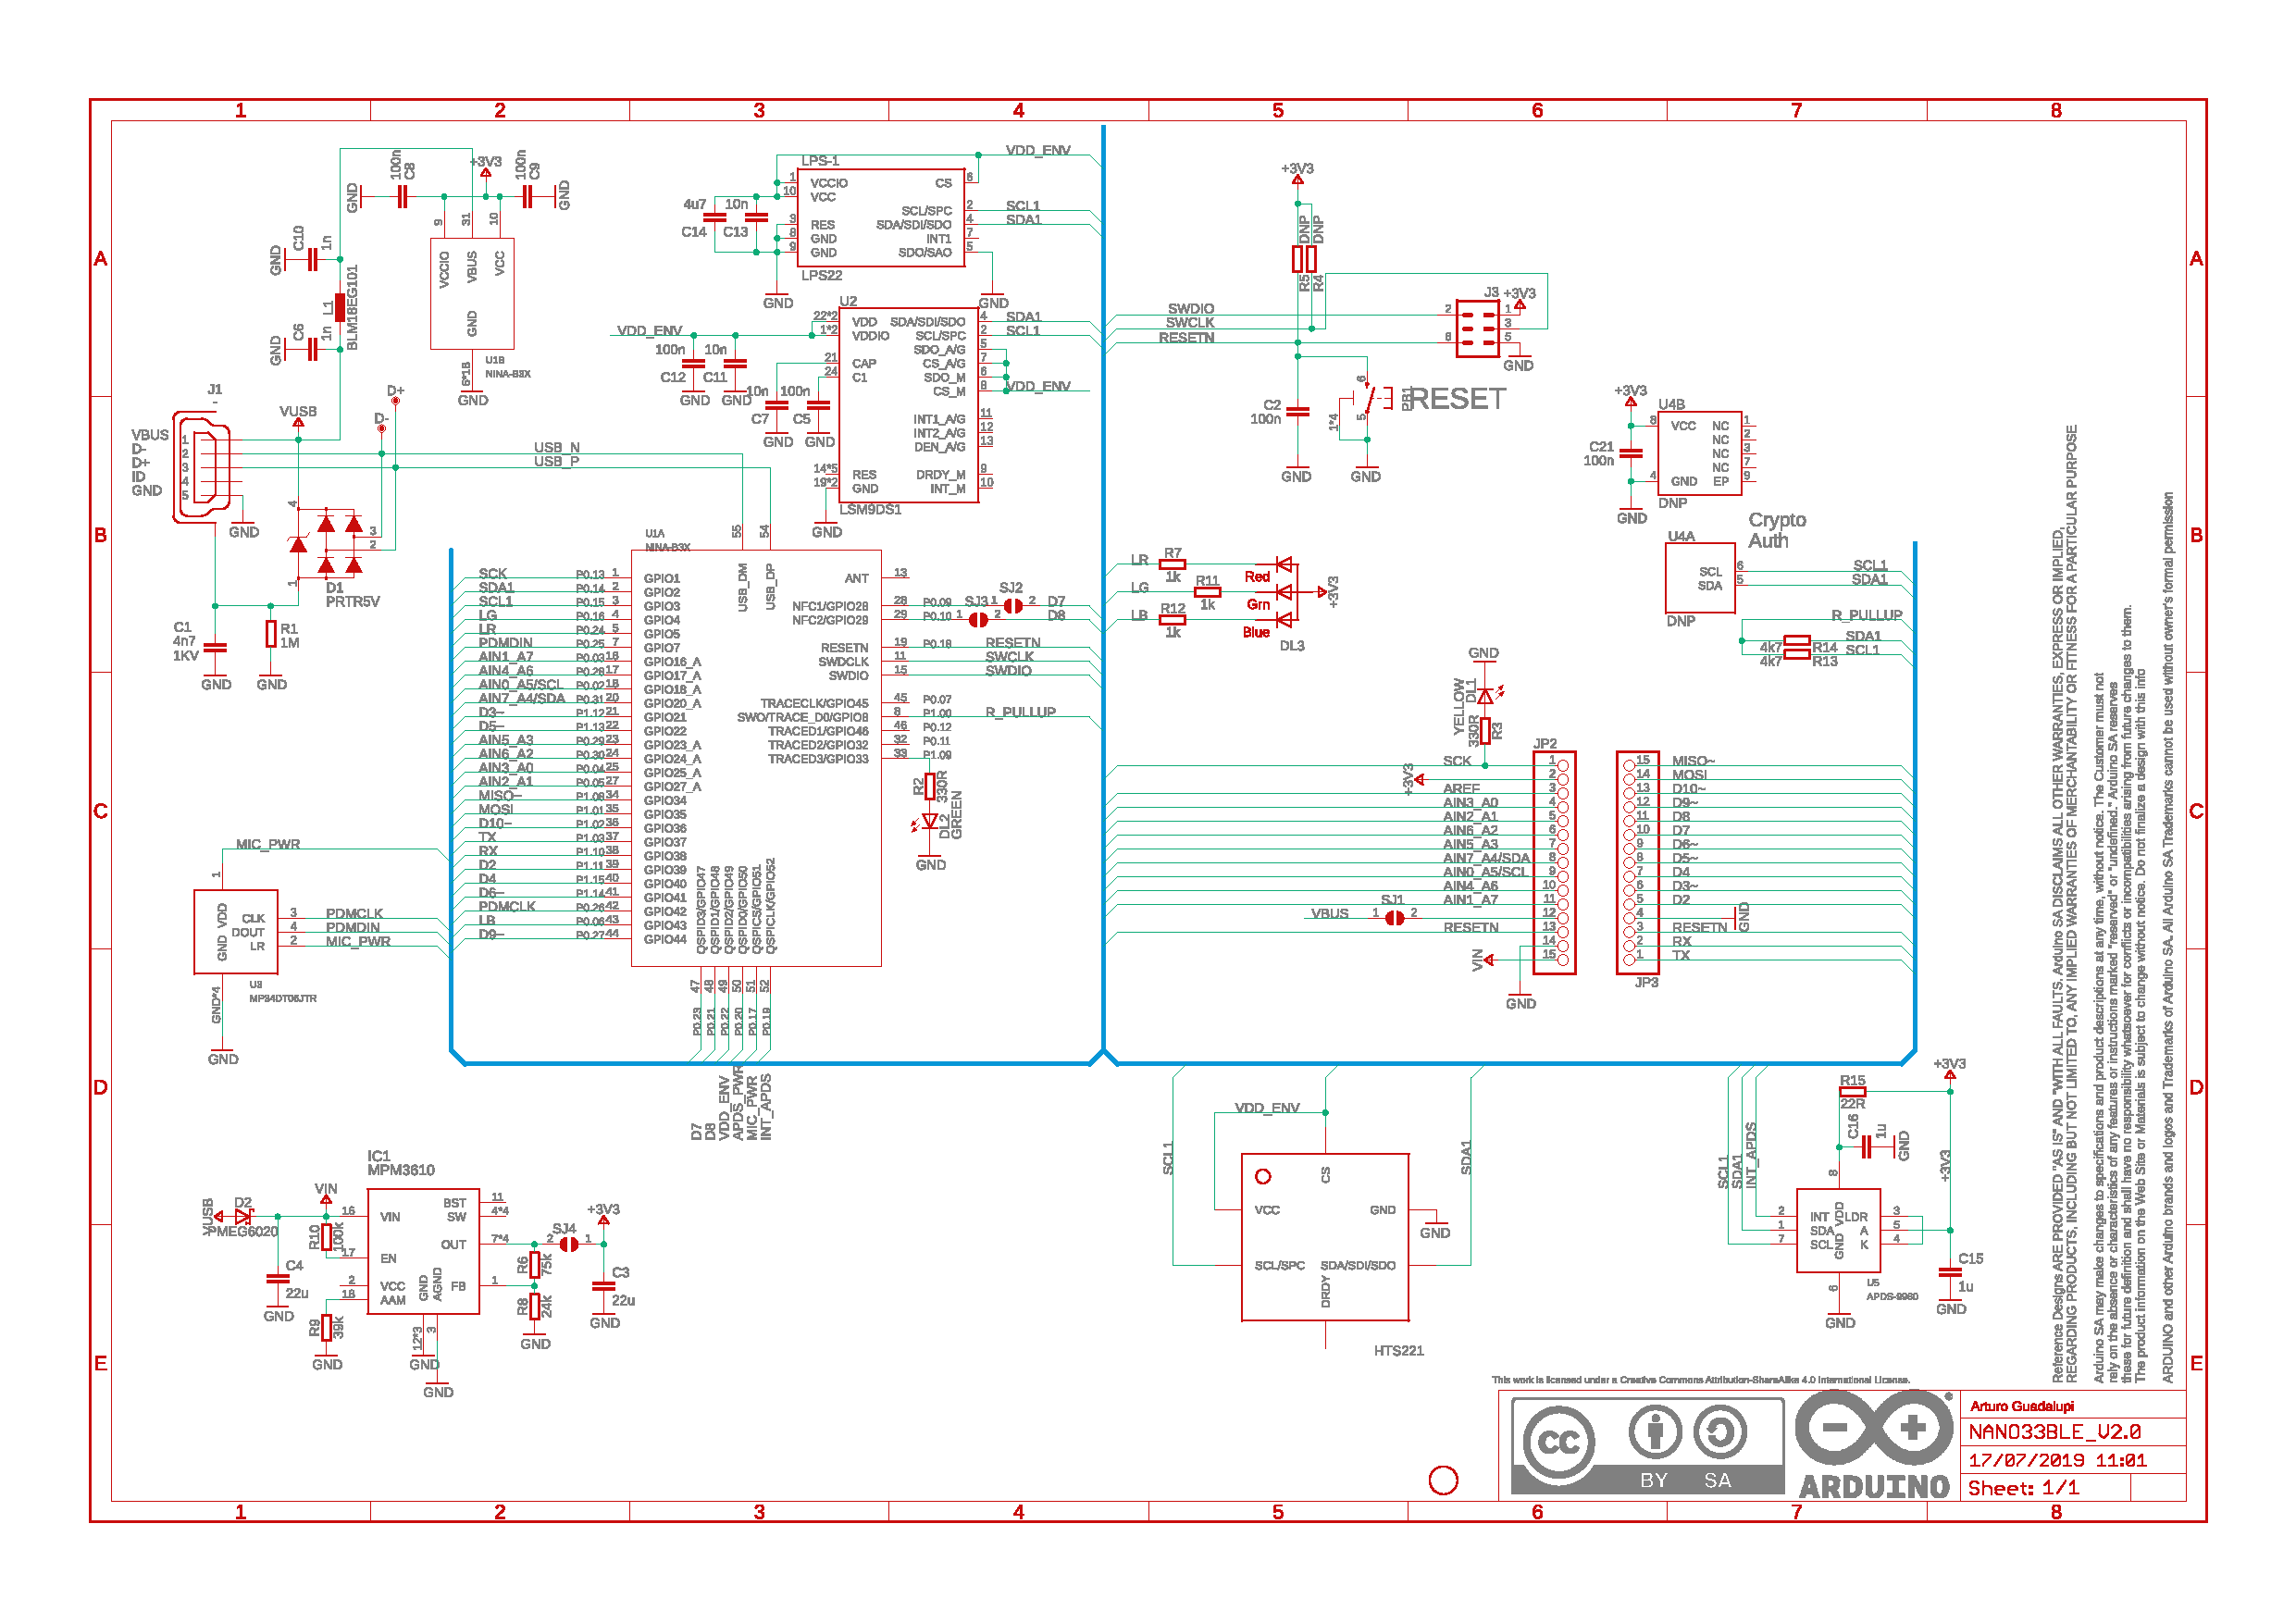
\includegraphics[width=\textwidth]{Documentos/NANO33BLE_V2.0_sch.pdf}
    \caption{Diagrama de bloques del CPU nRF52840. Fuente y créditos: \cite{nano33}.}
    \label{mcu-diagram}
\end{figure}


\subsubsection{Diagrama de pines}

\begin{figure}[H]
    \centering
    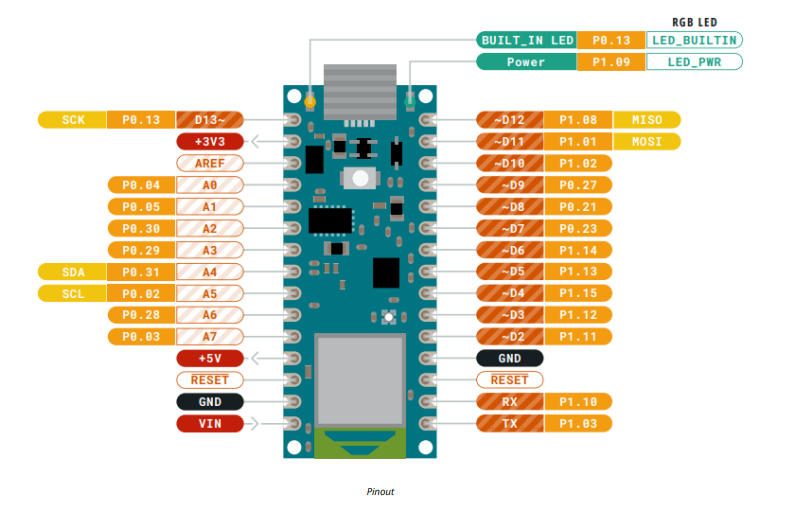
\includegraphics[width=\textwidth]{Imagenes/Arduino_Nano.png}
    \caption{Diagrama de pines del Arduino Nano BLE 33 Sense. Fuente y créditos: \cite{nano33}.}
    \label{pinout}
\end{figure}